% !TEX root =  free234.tex


\chapter{Vector Geometry in Three dimensional space}

\section{Three dimensional space}  
The world according to our first and second semester calculus courses is flat:
except for a brief digression about surfaces of revolution, everything that we
discussed in Math 221 and 222 took place in the $(x,y)$-plane.  All curves were
curves in the plane and all functions had graphs that were curves in the plane.
This semester we leave two dimensions behind and enter the three dimensional
world.  In order to understand the objects we will be dealing with, such as
curves that are free to loop around in space, or functions whose graphs are
themselves two dimensional curved surfaces, we will first review some three
dimensional geometry.  In particular, we will review the use of vectors in three
dimensional geometry.

\section{Geometric description of vectors}  
\label{sec:geometric-description-of-vectors}
\subsection{Points and their coordinates}  
We are used to describing the location of any point in the plane by choosing two
perpendicular ``coordinate axes'' (the $x$ and $y$ axes), and specifying the
corresponding $(x,y)$-coordinates of any given point.  In the same way we can
describe where points are in three dimensional space by choosing three mutually
perpendicular axes, which we call the $x$, $y$, and $z$ axes.  To say where some
given point $P$ is, we travel from the origin to $P$, first along the $x$ axis,
then parallel to the $y$-axis, and finally parallel to the $z$-axis.  The
distances we had to go in the $x$, $y$, and $z$ directions are the $x$, $y$, and
$z$ coordinates of our point $P$.

\begin{figure}[h]
  \centering
  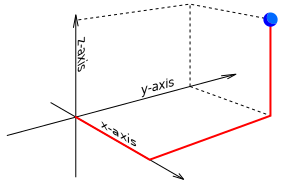
\includegraphics{01xyz-axes.pdf}
  \caption{To determine the location of points in three dimensional
    space (such as the center of the blue sphere in this drawing), we
    should choose three coordinate axes, and specify three numbers:
    the $x$, $y$, and $z$ coordinates of the point.  }
\end{figure}

\subsection{Vectors}  
While points and their coordinates are used to described locations in space,
vectors are used to describe \emph{displacements}, i.e.~how to go from one point
to another.  Such a displacement has a size (how far we have to go), and a
direction (which way do we go).  Vectors also get used in non-geometric
situations to describe objects that have size and direction, e.g.~velocities and
forces in physics are typical examples of vector-like objects.

\subsubsection*{Informal definition of ``vectors''}
We will think of a vector as an arrow connecting two points.  If the points are
$A$ and $B$ then we call the vector $\tpv AB$. If we translate a vector $\tpv
AB$ \emph{without turning it} then we say that the resulting vector $\tpv CD$ is
the same vector as the original vector $\tpv AB$.  A more precise way  of saying
that we should be able to move $\tpv AB$ ``without turning,'' is to insist that
the line segments $AB$ and $CD$ should be parallel, and have the same length and
orientation.

\begin{figure}[h]\centering
  \input ../figures/234/005equalvectors.tex
  \caption{This figure contains \emph{four} points ($A$, $B$, $C$, $D$),
  \emph{two} line segments ($AB$ and $CD$), but \emph{only one} vector since
  $\tpv AB$ and $\tpv CD$ represent the same vector:  $\tpv AB = \tpv CD$.}
\end{figure}
We say that the arrows $\tpv AB$ and $\tpv PQ$ \emph{both represent the same
vector.}  Since both $\tpv AB$ and $\tpv PQ$ are the same vector we will often
want to use a notation for vectors that does not emphasize any particular choice
of initial-~and endpoint.  The notation we will use in this course is
\[
\va = \tpv AB = \tpv PQ,
\]
i.e., a single letter with an arrow on top will always stand for a
vector in this course.

\begin{figure}[h]\centering
  \def\figfont{\sffamily\footnotesize\color{darkbluegreen}\centering}
  \def\addingvectorsCapA{\parbox{1in}{\figfont%
      to add\\
      two vectors\dots}} \def\addingvectorsCapB{\parbox{1in}{\figfont%
      \dots move one vector until its initial point\dots}}
  \def\addingvectorsCapC{\parbox{1in}{\figfont%
      \dots is the end point of the other\dots} }
  \def\addingvectorsCapD{\parbox{1in}{\figfont%
      \dots and combine them.} } \input
  ../figures/234/005adding-vectors2.pdf_tex
  \caption{Adding vectors}
\end{figure}
\section{Arithmetic of vectors}  
\label{sec:arithmetic-of-vectors}
To add two vectors $\tpv AB$ and $\tpv PQ$ we first translate the vector $\tpv
PQ$ so that its initial point becomes $B$; let the result of this translation be
the vector $\tpv BC$.  Then, by definition, the sum of $\tpv AB$ and $\tpv PQ$
is $\tpv AC$: in a formula,
\[
\tpv AB + \tpv PQ = \tpv AB + \tpv BC = \tpv AC.
\]
An equivalent way of adding two vectors $\tpv AB$ and $\tpv PQ$ is to move the
vectors around until they have the same initial point.  Two vectors with a
common initial point form two sides of a parallelogram (see
Figure~\ref{fig:adding-vectors-parallelogram}) and the sum of the two vectors is
the diagonal of that parallelogram.
\begin{figure}[h]
  \input ../figures/234/005adding-vectors-parallelogram.pdf_tex
  \caption{{\bfseries Using a parallelogram to add vectors. } To find $\tpv AB +
  \tpv AD$ we move the vector $\tpv AD$ so that its initial point is at $B$,
  i.e.~the endpoint of $\tpv AB$.  This gives us a parallelogram $ABCD$, where
  $\tpv AD = \tpv BC$.  Therefore $\tpv AB+\tpv AD = \tpv AB+\tpv BC = \tpv AC$
  }
  \label{fig:adding-vectors-parallelogram}
\end{figure}

One can also multiply vectors with numbers.  To multiply a vector $\va$ with a
positive real number $t>0$, we multiply the length of the vector by a factor
$t$, without changing the direction of the vector.
\begin{figure}[h]
  \input ../figures/222/05scalar-mult.pdf_tex
  \caption{Multiplying and subtracting vectors}
\end{figure}
\section{Vector algebra}  
The addition and multiplication of vectors and numbers satisfy a number of
algebraic properties that should look familiar, as they are very similar to the
usual algebraic properties for adding and multiplying numbers.  Here they are:
\begin{align*}
  \va+\vb&=\vb+\va &&& \text{commutative law}\\
  (\va+\vb)+\vc &= \va+(\vb+\vc) & t\cdot(s\cdot\va) &= (ts)\cdot \va
  &\text{associative laws}\\
  t\cdot(\va+\vb) & = t\va+t\vb & (t+s)\va &= t\va + s\va
  &\text{distributive laws}
\end{align*}
\section{Component representation of vectors}  
\label{sec:component-rep-of-vectors}

\subsection{Components of a vector in two dimensional space}  
\label{sec:comp-vect-two}
There is a way to represent a vector by specifying a list of numbers instead of
by giving a geometric description of the vector.  To do this for vectors in the
plane, we must choose two perpendicular coordinate axes (the ``$x$'' and ``$y$''
axes).  We define
\begin{align*}
  \ves1 &= \text{ vector with length $1$, in the direction of the $x$ axis} \\
  \ves2 &= \text{ vector with length $1$, in the direction of the $y$ axis}
\end{align*}
Then any other vector can be written as the sum of a multiple of $\ves1$ and
another multiple of $\ves2$:
\begin{equation}
  \va = a_1\ves1 + a_2 \ves2.
  \label{eq:vector-a-in-components}
\end{equation}
See Figure~\ref{fig:vector-in-components}.  The numbers $a_1$ and $a_2$ are
called the \emph{components of the vector $\va$.}  If we know the components
$a_1$ and $a_2$ of a vector, and if we know the two vectors $\ves1$ and $\ves2$,
then we can reconstruct the vector $\va$ by using the formula
\eqref{eq:vector-a-in-components}.

\begin{figure}[h]
  \input{../figures/234/005vector-components.pdf_tex}
  \caption{Describing a vector in terms of its components.}
  \label{fig:vector-in-components}
\end{figure}

Instead of using the notation \eqref{eq:vector-a-in-components}, one very often
writes
\begin{equation}
  \va = \vek a_1 \\ a_2 \tor,
  \text{ or }
  \va = \begin{bmatrix}
    a_1 \\ a_2
  \end{bmatrix}, \text{ or } \va = \langle a_1, a_2\rangle.
  \label{eq:vector-a-as-column-vector}
\end{equation}
This notation says that $\va$ is the vector whose components are $a_1$ and
$a_2$.  Since the two vectors $\ves1$ and $\ves2$ depend on our choice of
coordinate axes, we can only use the component notation if it is clear to
everyone how we chose the coordinate axes.

The first way of writing the vector, in which the components $a_1$ and $a_2$ are
listed in a column enclosed in either parentheses or square brackets, is the
standard way of writing ``column vectors,'' and is used in linear algebra
courses (math 320, 340, 341, etc.), as well as by most computational software
(Matlab$^{\rm TM}$, Octave, etc.).  The other way of writing the components,
i.e.~as $\langle a_1, a_2\rangle$, also
gets used, especially when one has to type the equations rather than write them
by hand.

\subsection{Components of a vector in three dimensional space}  
\label{sec:comp-vect-three}
The preceding also applies to vectors in three dimensional space: instead of
choosing two coordinate axes we choose three axes, and call them the $x$, $y$,
and $z$ axes (or, the $x_{1}$, $x_{2}$, and $x_{3}$ axes).  Then we define
$\vi$, $\vj $, and $\vk$ (or $\ves1$, $\ves2$, and $\ves3$) to be vectors of
length one in the direction of the three coordinate axes.  A vector $\va$ in
space can then be written as a combination of the three vectors $\vi$, $\vj$,
and $\vk$, namely,
\[
 \va = a_{1}\vi + a_2 \vj + a_3 \vk, \text{ or }
 \va = \vek a_1\\a_2\\a_3 \tor.
\]
\begin{figure}[h]
  \sffamily\color{darkbluegreen}
  \input{../figures/234/005vector-components3D.pdf_tex}
  \caption{Components of a vector in three dimensional space}
  \label{fig:vector-in-components-3d}
\end{figure}%
\marginpar{\centering\dfnt Josiah Willard Gibbs\\
1839--1903\\[2pt]
%\includegraphics[width=1in]{Josiah_Willard_Gibbs.jpg}\\
\tiny\url{https://en.wikipedia.org/wiki/Josiah_Willard_Gibbs}}%
The $\ves1$, $\ves2$, $\ves3$ notation is more systematic, but the $\vi$, $\vj$,
$\vk$ notation, which was introduced into vector geometry and vector calculus by
J.W.Gibbs, is also very common.

\subsection{Length of a vector whose components are given}  
\label{sec:length-vector-given-components}
We will write
\[
\|\va\|
\]
for the length of a vector $\va$.  If the vector is given in components, 
\[
  \va = a_1\ves1+a_2\ves2, 
  \text{ or }
  \va = a_1\ves1+a_2\ves2+a_3\ves3, 
\]
then the length of the vector is determined by Pythagoras' law (see
Figures~\ref{fig:vector-in-components} and~\ref{fig:vector-in-components-3d}):
\begin{equation}
  \|\va\| = \sqrt{a_1^2 + a_2^2}, \quad
  \text{ or }\quad
  \|\va\| = \sqrt{a_1^2 + a_2^2+a_3^2}. 
  \label{eq:length-of-vector-from-components}
\end{equation}



\section{The dot product}  
There are two different descriptions of the dot product of two
vectors: one geometric, and the other in terms of the components of
the vectors.

\subsection{Geometric description of the dot product}  
If $\va$ and $\vb$ are two given vectors, then, by definition,
\marginpar{\footnotesize\sffamily\centering\color{darkbluegreen}%
  \input ../figures/234/005dot-product.pdf_tex

  The dot product between two vectors.
}
\begin{equation}
  \label{eq:dotproduct-geometric}
  \va\dpp\vb = \|\va\| \, \|\vb\|\,\cos \theta,
\end{equation}
where $\theta$ is the angle between the two vectors $\va$ and $\vb$.

\subsection{The dot product in terms of vector components}  
If we choose an orthonormal set of vectors $\ves1,\ves2,\ves3$, and write
\[
  \va = a_1\ves1+a_2\ves2+a_3\ves3=\vek a_1 \\ a_2 \\ a_3 \tor,\qquad
  \vb = b_1\ves1+b_2\ves2+b_3\ves3=\vek b_1 \\ b_2 \\ b_3 \tor,
\]
then
\begin{equation}
  \label{eq:dotproduct-algebraic}
  \va\dpp\vb = a_1b_1 + a_2b_2 + a_3b_3.
\end{equation}
The fact that \eqref{eq:dotproduct-geometric} and \eqref{eq:dotproduct-algebraic}
always give the same result is not obvious (the formulas look very different), and
requires a proof.  A very common proof relies on the law of cosines (it was given in math 222 -- see also Problem~\ref{prb:law-of-cosines-and-dotprod})

\subsection{Algebraic properties of the dot product}  
\label{sec:dotproduct-algebraic-properties}%
The dot product has the following algebraic properties, which we will
use very often throughout this course:
\begin{align*}
  \va\dpp\vb &= \vb\dpp\va & \text{commutative} \\
  s(\va\dpp\vb) &= (s\va)\dpp\vb & \text{associative} \\
  (\va+\vb)\dpp\vc & = \va\dpp\vc + \vb\dpp\vc. & \text{distributive}
\end{align*}
We will not prove these properties here.  Proofs can be given if one
starts either from the algebraic description of the dot-product
\eqref{eq:dotproduct-algebraic}, or from the geometric description
\eqref{eq:dotproduct-geometric} (although the distributive property is
more difficult to prove from the geometric description than from the
algebraic description.)

The sign of the dot product tells us if the angle between two vectors is acute,
obtuse, or if the vectors are perpendicular:
\begin{subequations}
  \begin{align}
    \va\perp\vb  &\iff \va\dpp\vb=0 \\
    \va\dpp\vb>0 &\iff \theta<\frac{\pi}{2}\\
    \va\dpp\vb<0 &\iff \theta>\frac{\pi}{2}.
  \end{align}
\end{subequations}

\section{The cross product}  
As with the dot product, the cross product of two vectors also has a
geometric description, and a description in terms of components.

\subsection{Geometric description of the cross product} Let $\va$  
and $\vb$ be two vectors in three dimensional space, then their
\emph{cross product} is the vector $\va\cp\vb$ that satisfies
\begin{itemize}
\item $\va\cp\vb$ is perpendicular to $\va$, and also to $\vb$
\item the length of $\va\cp\vb$ is given by
  \[
  \|\va\cp\vb\| = \|\va\|\,\|\vb\|\,\sin\theta,
  \]
  where $\theta$ is the angle between the vectors $\va$ and $\vb$,
\item the three vectors $\va$, $\vb$, $\va\cp\vb$ satisfy the
  \emph{right hand rule:} if on your right hand $\va$ is the index
  finger and $\vb$ is the middle finger, then your thumb points in the
  direction of $\va\cp\vb$.  See Figure~\ref{fig:cross-product}.
\end{itemize}
\begin{figure}[t]
  \input ../figures/222/05crossprod-corkscrew.pdf_tex
  \caption{The cross product: $\va\cp\vb$ is perpendicular to both
    $\va$ and $\vb$; its direction follows from the right-hand rule. }
  \label{fig:cross-product}
\end{figure}
The length of the cross product of two vectors has a geometric
interpretation.  Namely, the quantity $\|\va\|\,\|\vb\|\,\sin\theta$
is exactly the are of the parallelogram spanned by the vectors $\va$
and $\vb$.
\begin{figure}[h]
  \input
  ../figures/222/05area-parallelogram-spanned-by-vectors.pdf_tex
\end{figure}

\subsection{Algebraic description of the cross product} If $\va$  
and $\vb $ are given by \eqref{eq:dotproduct-geometric}, i.e.~by
\[
\va = a_1\ves1+a_2\ves2+a_3\ves3=\tvek a_1 \\ a_2 \\ a_3 \ttor,\qquad
\vb = b_1\ves1+b_2\ves2+b_3\ves3=\tvek b_1 \\ b_2 \\ b_3 \ttor,
\]
then
\[
\va \cp\vb = \vek
a_2b_3 - a_3b_2\\
a_3b_1 - a_1b_3\\
a_1b_2 - a_2b_1\tor.
\]

\subsection{Algebraic properties of the cross product}  
\label{sec:cross-product-algebraic-properties}
The cross product has the distributive property, namely,
\begin{equation}
  (\va+\vb)\cp\vc  = \va\cp\vc + \vb\cp\vc,
  \label{eq:cross-product-distributive}
\end{equation}
holds true for any three vectors $\va$, $\vb$, $\vc$.

The cross product is \emph{not commutative}: $\va\cp\vb$ and
$\vb\cp\va$ are not the same thing.  Instead, we have :
\begin{equation}
  \va\cp\vb = -\vb\cp\va.
\end{equation}
Because of this property the cross product is said to be
``\textit{anti-commutative.}''

The associative property fails completely for the cross product: for
most vectors $\va$, $\vb$, $\vc$ one has
\begin{equation}\color{red}
  \carefulnow\carefulnow\qquad
  (\va\cp\vb)\cp\vc\; {\boldsymbol \neq}\; \va\cp(\vb\cp\vc)
  \qquad \carefulnow\carefulnow
  \label{eq:cross-product-not-associative}
\end{equation}

If you need a vector that is perpendicular to two given vectors, take
their cross product.

The length of the cross product $\va\cp\vb$ is the area of the
parallelogram spanned by those vectors.

\section{The triple product}  
\label{sec:determ-triple-prod}
Just as two vectors in the plane form a parallelogram, three vectors
in space will form a shape called a parallelepiped.  By definition, a
parallelepiped is a solid body each of whose faces is a parallelogram.

\begin{figure}[h]
  \def\svgwidth{200pt}
  \input ../figures/234/01parallelepiped.pdf_tex\hfill
  \def\svgwidth{130pt}
  \input ../figures/234/01parallelepiped-flipped.pdf_tex
  \caption{\textbf{A parallelepiped spanned by three vectors $\va$,
      $\vb$, $\vc$.}  Since the base of the parallelepiped is a
    parallelogram with edges $\vb$ and $\vc$, we have \\
    \null\qquad Area of base~$= \|\vb\cp\vc\|$.\\
    The height of the parallelepiped is $\|\va\|\cos\theta$, and
    therefore the volume is given by \\
    \null\qquad Volume = $\text{height}\cdot\text{area of base}
    = \|\va\| \, \|\vb\cp\vc\| \cos\theta
    = \va\dpp\bigl(\vb\cp\vc\bigr)$.\\
    This derivation applies to the situation on the left, where the
    vector $\va$ and the cross product $\vb\cp\vc$ point in the same
    direction.  If these vectors form an obtuse angle, as is the case
    on the right, then $\cos\theta<0$, and the height is
    $-\|\va\|\cos\theta$.  In that case one has\\
    \null\qquad Volume = $\text{height}\cdot\text{area of base}
    = - \|\va\| \, \|\vb\cp\vc\| \cos\theta 
    = - \va\dpp\bigl(\vb\cp\vc\bigr)$.
  }
  \label{fig:volume-of-parallelpiped}
\end{figure}
If we are given three vectors $\va$, $\vb$, and $\vc$, then the volume
of the parallelepiped they determine is given by the formula
\[
\text{``Volume equals Area of base times height''}
\]
In terms of the three vectors this is
\begin{equation}
  V = \left| \va\dpp\bigl(\vb\cp\vc\bigr)\right|.
  \label{eq:volume-of-parallelpiped}
\end{equation}
A derivation is sketched in Figure~\ref{fig:volume-of-parallelpiped}.
The quantity $\va\dpp(\vb\cp\vc)$ (without the absolute values) is
called the \emph{triple product} of the three vectors $\va$, $\vb$,
and $\vc$.  Apart from its use in computing the volume of a
parallelepiped, the triple product appears in many other contexts.  At
first sight the expression $\va\dpp(\vb\cp\vc)$ suggests that the
order in which the vectors appear is important, but this turns out not
to be true.  One has 
\[
\va\dpp\bigl(\vb\cp\vc\bigr) = \vb\dpp\bigl(\vc\cp\va\bigr) =
\vc\dpp\bigl(\va\cp\vb\bigr)
\]
for any $\va,\vb,\vc$.

\section{Determinants}  
\label{sec:determinants}
For any four numbers $a$, $b$, $c$, $d$, one defines the $2\times2$
determinant to be
\begin{equation}
  \deter a&b \\ c& d
  \minant
  =ad-bc\,.
  \label{eq:determinant-2x2}
\end{equation}
One can also define $3\times3$ determinants.  Namely, for any nine
numbers $a_1, \dots, c_3$ one defines
\begin{equation}
  \deter
      a_1 & b_1 & c_1 \\
      a_2 & b_2 & c_2 \\
      a_3 & b_3 & c_3
  \minant
  =
  a_1b_2c_3 - a_1b_3c_2 - a_2b_1c_3 + a_2b_3c_1 +a_3b_1c_2 - a_3b_2c_1\,.
  \label{eq:triple-product}
\end{equation}
This can be written as
\begin{align}
  \deter
  \color{red}a_1 & b_1 & c_1 \\
  \color{red}a_2 & b_2 & c_2 \\
  \color{red}a_3 & b_3 & c_3
  \minant
  &={\color{red}a_1}\bigl(b_2c_3-b_3c_2\bigr)
  - {\color{red}a_2}\bigl(b_1c_3-b_3c_1\bigr)
  + {\color{red}a_3}\bigl(b_1c_2-b_2c_1\bigr)
  \label{eq:determinant-expanded-along-column}
  \\
  &= {\color{red}a_1} \deter b_2 & c_2 \\ b_3 & c_3 \minant
  - {\color{red}a_2} \deter b_1 & c_1 \\ b_3 & c_3 \minant
  + {\color{red}a_3} \deter b_1 & b_1 \\ b_2 & b_2 \minant
  \notag
\end{align}
where each coefficient in the first row is multiplied with the
$2\times2$ determined that remains after one deletes the row and
column containing the coefficient.

Instead of expanding along the first row one can also expand along the
first column:
\begin{equation}
  \deter
  \color{red}a_1 & \color{red}b_1 & \color{red}c_1 \\
  a_2 & b_2 & c_2 \\
  a_3 & b_3 & c_3
  \minant
  = {\color{red}a_1}\deter b_2 & c_2 \\ b_3 & c_3 \minant
  - {\color{red}b_1}\deter a_2 & c_2 \\ a_3 & c_3 \minant
  + {\color{red}c_1}\deter a_2 & b_2 \\ a_3 & b_3 \minant
  \label{eq:determinant-expanded-along-row}
\end{equation}
Many other mnemonic devices exist to remember how to compute a
$3\times3$ determinant.  A popular trick is ``Sarrus' rule'' (see
Figure~\ref{fig:Sarrus}.)

One can also define larger determinants, i.e.~$4\times4$, $5\times5$,
etc, and generally $n\times n$ determinants.  The theory, which is
beyond the scope of this course, is treated in linear algebra courses
such as Math 320, 340, or 341.

\section{Determinants, the triple product, and the cross product}  
\label{sec:determ-triple-prod-cross-prod}
If the numbers $a_1, \dots, c_3$ in a determinant happen to be the
components of three vectors $\va$, $\vb$, $\vc$, i.e.~if
\[
\va = \vek a_1\\ a_2 \\a_3\tor, \vb = \vek b_1\\ b_2 \\b_3\tor, \vc =
\vek c_1\\ c_2 \\c_3\tor,
\]
then the corresponding determinant is exactly the triple product:
\begin{equation}
  \left|
    \begin{array}{ccc}
      a_1 & b_1 & c_1 \\
      a_2 & b_2 & c_2 \\
      a_3 & b_3 & c_3
    \end{array}
  \right|= \va\dpp\bigl(\vb\cp\vc\bigr).
\end{equation}%
\begin{figure}[t]
  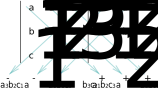
\includegraphics[scale=1.30]{05determinant-shortcut2.pdf}
  \caption{\textbf{Computing $3\times3$ determinants. } There are several
    shortcuts to remember how to compute a $3\times3$ determinant.
    Pictured here is ``Sarrus' rule,'' which tells us to copy the
    first two columns of the determinant to the right of the
    determinant, and read off the six terms in the determinant by
    following the diagonals. }
  \label{fig:Sarrus}
\end{figure}%
Related to this is the following practical trick for computing the
cross product of two column vectors.  Given two column vectors $\vb$
and $\vc$ one can write their cross product as 
\begin{align*}
  \vek b_1\\b_2\\b_3\tor\cp \vek c_1\\c_2\\c_3\tor
  &=
  \deter
  \ves1 & b_1 & c_1 \\
  \ves2 & b_2 & c_2 \\
  \ves3 & b_3 & c_3
  \minant \\
  &=  \deter b_2 & c_2 \\ b_3 & c_3 \minant \ves1
    - \deter b_1 & c_1 \\ b_3 & c_3 \minant \ves2
    + \deter b_1 & c_1 \\ b_2 & c_2 \minant \ves3 .
\end{align*}
The $3\times3$ determinant in this equation is unusual in that some of its
entries are vectors instead of numbers.  The intention of this notation is that
one expand the determinant along the first column, as in
\eqref{eq:determinant-expanded-along-column} and then interpret the result as a
vector.

\section{Defining equations for lines and planes}  
\label{sec:defining-equations-lines-and-planes}
\subsection{Lines}  
\label{sec:defining-eq-lines}
Let $\ell$ be a line in the plane, and suppose we know one point $A$ on the
line, and that we also have a vector $\vn$ that is perpendicular to the line
(and we exclude $\vn=\vvv0$.) Such a vector is called a \emph{normal vector} to
the line.  Given any other point $X$ in the plane we can form the vector $\tpv
AX$ and consider its dot-product with the normal.  We have
\[
  \vn \dpp \tpv AX = \|\vn\| \, \|\tpv AX\| \cos \theta,
\]
where $\theta$ is the angle between the normal vector $\vn$ and $\tpv AX$.

\begin{figure}[h]
  \hspace{-1em}\input ../figures/222/05distance-to-line.pdf_tex
\end{figure}
The combination $\|\tpv AX\|\cos \theta$ is, up to its sign, the distance from
the line $\ell$ to the point $X$: If $X$ lies on the side of $\ell$ at which the
normal vector points then $\vn\dpp\tpv AX>0$; if $X$ lies on the other side then
$\vn\dpp\tpv AX<0$.  We therefore have the following formula for \textit{the
distance between a point $X$ and the line $\ell$:}
\begin{equation}
  d = \frac{\vn \dpp \tpv AX	}{\|\vn\|}
  \label{eq:distance-to-line}
\end{equation}
When we use this equation to compute the distance from $X$ to $\ell$, it is good
to recall that if $\vx=\tvek x_1\\x_2\ttor$ and $\va = \tvek a_1\\ a_2\ttor$ are
the position vectors of the points $X$ and $A$, then  
\[
  \tpv AX = \vx-\va = \vek x_1-a_1 \\ x_2-a_2\tor.
\]
Moreover, the length of the normal vector is $\|\vn\| = \sqrt{n_1^2+n_2^2}$, so
we can rewrite \eqref{eq:distance-to-line} as 
\[
  d = \frac{n_1(x_1-a_1) + n_2(x_2-a_2)}{\sqrt{n_1^2 + n_2^2}}.
\]
This last formula is more impressive than \eqref{eq:distance-to-line}, but it is
better to remember \eqref{eq:distance-to-line}.

The equation for the distance from any point $X$ to a given line $\ell$ is also
important because it gives us \emph{the defining equation} for the line $\ell$.
The defining equation is an equation that tells us for any given point $X$ in
the plane if that point is on the line or not.  Since $X$ is on $\ell$ exactly
when the distance from $\ell$ to $X$ vanishes, it follows from
\eqref{eq:distance-to-line} that $X$ is on $\ell$ if and only if 
\begin{equation}
  \vn\dpp\tpv AX = 0.
  \label{eq:defining-eqn-for-line}
\end{equation}
We can again rewrite this equation in a few different ways.  If we want to write
it in terms of the position vectors of $A$ and $X$, then we get
\[
  \vn \dpp \bigl(\vx-\va\bigr) = 0, \qquad
  \text{ i.e.: }\qquad
  \vn\dpp\vx = \vn\dpp\va.
\]
Written without vectors, but in terms of the coordinates of the points $A$,
$X$, and the components of the normal vector $\vn$, we can write this last
version of our equation as
\[
  n_1x_1+n_2x_2 = n_1a_1+n_2a_2.
\]

\subsection{Planes}  
\label{sec:defining-eq-planes}
We can repeat the derivation of the distance from a point to a line in
the plane and derive a formula for the distance from a point in three
dimensional space to a given plane.  The drawings are harder to make
(at first only, practice makes perfect!), but the resulting formulas
are the same.
\begin{figure}[h]
  \centering
  \input ../figures/234/01distance-to-plane.pdf_tex
\end{figure}

The distance from a point $X$ to a plane $\cP$ is given by equation
\eqref{eq:distance-to-line}, where $\vn$ is a normal vector to the
plane (a vector that is perpendicular to the plane), and $A$ is some
point on the plane that we happen to know.


\section{Problems}  
%\begin{multicols}{2}
\problemfont  
\problem \subprob Simplify the following 
\begin{align*}
  \va &= \vek 1\\-2\\3 \tor + 3\vek 0 \\ 1 \\3 \tor &
  \vb &=  12\vek 1 \\ 1/3\tor - 3\vek 4 \\ 1\tor \\
  \vc &= (1+t)\vek 1 \\ 1-t\tor - t\vek 1 \\ -t\tor &
  \vd &= t\vek1\\0\\0\tor + t^2\vek0\\-1\\2\tor-\vek0\\0\\1\tor
\end{align*}
\subprob Write the vectors from part \textbf{(a)} using Gibbs' notation, i.e.~write
them in terms of $\vi$, $\vj$, $\vk$.   (See \S~\ref{sec:component-rep-of-vectors}).

\problem If $\va,\vb, \vc$ are as in the previous problem, then 
which of the following expressions mean anything? Compute those
expressions that are well defined.
\begin{align*}
  \tsubprob& \va+\vb  &\tsubprob& \vb+\vc &\tsubprob& \pi\va \\
  \tsubprob& \vb^2    &\tsubprob& \vb/\vc &\tsubprob& \nm\va+\nm\vb \\
  \tsubprob& \nm\vb^2 &\tsubprob& \vb/\nm\vc &&
\end{align*}

\problem Let $\va=\tvek1\\-2\\2\ttor$ and $\vb=\tvek 2\\-1\\1\ttor$.
\quad Compute:
\begin{align*}
&\tsubprob ||\va||&&
\tsubprob 2\va&&
\tsubprob ||2\va||^2\\
&\tsubprob \va+\vb&&
\tsubprob 3\va-\vb&&
\end{align*}
\vskip-2ex
\answer  
(a) $3$ \quad
(b) $\tvek 2\\ -4\\ 4\ttor$  \quad
(c) 36  \quad
(d) $\tvek 3\\ -3\\ 3\ttor$  \quad
(e) $\tvek 1\\ -5\\ 5\ttor$
\endanswer

\problem Given: points $A (2,1)$ and $B (-1,4)$.  Compute the vector $\tpv AB$.
\textit{Is $\tpv AB$ a position vector?}
\answer 
Every vector is a position vector.  To see of which point it is the position
vector translate it so its initial point is the origin.

Here $\tpv AB = \vek -3\\ 3 \tor$, so $\tpv AB$ is the position vector of
the point $(-3,3)$.
\endanswer

\problem Given: points $A (2,1)$, $B (3,2)$, $C (4,4)$ and $D (5,2)$.\\
Question: \textit{Is $ABCD$ a parallelogram?}
\answer 
One always labels the vertices of a parallelogram counterclockwise (see
\S\ref{sec:diag-parall}). 

$ABCD$ is a parallelogram if $\tpv AB + \tpv AD = \tpv AC$.  
$\tpv AB = \vek 1\\ 1 \tor$, $\tpv AC = \vek 2\\ 3 \tor$, $\tpv AD = \vek 3\\
1 \tor$.  So $\tpv AB + \tpv AD \ne \tpv AC$, and $ABCD$ is not a
parallelogram.
\endanswer

\problem Given: points $A (0,2,1)$, $B (0,3,2)$, $C (4,1,4)$ and $D$.

\subprob If $ABCD$ is a parallelogram, then what are the coordinates of
the point $D$?
\answer 
As in the previous problem, we want $\tpv AB + \tpv AD = \tpv AC$.
If $D$ is the point $(d_1, d_2, d_3)$ then 
$\tpv AB = \vek 0\\ 1\\1 \tor$, 
$\tpv AD = \vek d_1\\ d_2-2 \\ d_3-1\tor$,
$\tpv AC = \vek 4\\ -1\\ 3 \tor$,
so that $\tpv AB + \tpv AD = \tpv AC$ will hold if 
$d_1 = 4$, $d_2 = 0$ and $d_3 = 3$.
\endanswer

\subprob If $ABDC$ is a parallelogram, then what are the coordinates of
the point $D$?
\answer 
Now we want $\tpv AB + \tpv AC = \tpv AD$, so $d_1 = 4$, $d_2 = 2$,
$d_3 = 5$.
\endanswer

\problem You are given three points in the plane: $A$ has coordinates $(2,3)$, $B$
has coordinates $(-1,2)$ and $C$ has coordinates $(4,-1)$.

\subprob Compute the vectors $\tpv AB$, $\tpv BA$, $\tpv AC$, $\tpv CA$, $\tpv
BC$ and $\tpv CB$.

\subprob Find the points $P, Q, R$ and $S$ whose position vectors are $\tpv AB$,
$\tpv BA$, $\tpv AC$, and $\tpv BC$, respectively.  \textit{Make a precise
drawing.}

\problem Explain how you can use the dot product to find the angle  
between the vectors $\va = 2\vi-3\vj$, and $\vb=\vj+\vk$.

\problem For which value(s) of the number $s$ are the vectors  
\[
\va =\vek s \\1-s\tor \text{ and }
\vb = \vek 2\\3\tor
\]
perpendicular?  For which values of $s$ do they make an acute angle?
\answer  
Compute the dot product: $\va\dpp\vb = 2s+3(1-s) = 3-s$.  When the
dot-product vanishes the vectors are perpendicular; this happens when
$s=3$.  The angle between the vectors is acute is the dot-product is
positive.  This happens when $3-s>0$, i.e.~when $s<3$.
\endanswer


\begin{figure}[t] 
  \centering
  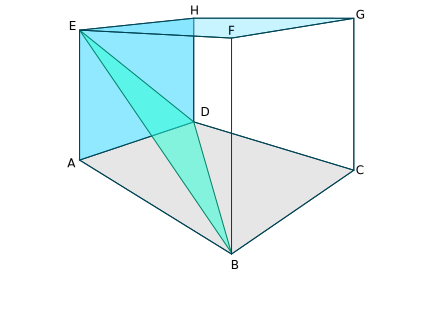
\includegraphics[width=0.75\textwidth]{01problem-cube-planes-angles.pdf}  
  \caption{Figure for problem \ref{prb:cube-planes-angles}}
  \label{fig:cube-planes-angles}  
\end{figure}
\problem\label{prb:cube-planes-angles} Figure  
\ref{fig:cube-planes-angles} shows a cube whose sides have length 1.

Choose $A$ to be the origin, and let the $x$, $y$, and $z$ axes be
along the sides $AB$, $AD$, and $AE$, respectively.

\subprob Draw the vectors $\ves1$, $\ves2$, and $\ves3$ in the figure.  

\subprob Find a normal vector to the plane through the points $B$,  
$D$, and $E$.

\subprob Draw the plane through $ACH$ (or at least the portion of that  
plane that lies inside the cube).  Find a normal to the plane $ACH$.

\subprob Find the angle between the two planes $BDE$ and $ACH$.  
(The angle between two planes is the same as the angle between their normal
vectors, i.e.~to find the angle between two planes find a normal vector for each
of the planes and compute the angle between these two vectors.)

\subprob Find the angle between the two planes $BDE$ and $HFC$.  

\problem \subprob Draw two vectors $\va$ and $\vb$ for which  
$\va$ has length 3, $\vb$ has length $5$, and for which $\va\dpp\vb=-12$.
\answer  
The problem is open-ended because it doesn't specify what ``draw'' means.

If you are allowed to use a calculator and a protractor, then you could use the
dot product to compute the angle $\theta$ between the two vectors; then, using
your protractor, draw two line segments that make this angle, and mark off
lengths 3 and 5 to get the vectors.  From the dot-product and the two lengths
you find $3\times5\times\cos\theta = -12$, so $\cos\theta = - \frac{12}{15}=
-0.8$, which implies $\theta = \arccos (-0.8) \approx 2.498\dots$ radians, or
$\theta\approx 143.13\dots$ degrees.

A different approach goes like this.  Suppose $\va$ is parallel to the $x_1$ axis; since $\va$ has length $3$, we can choose $\va=3\ves1$.  Now we look for a matching vector $\vb=\tvek b_1\\b_2\ttor$.  The condition that $\vb$ must have length 5
then says $b_1^2 + b_2^2 = 5^2 = 25$, while the dot-product is $\va\dpp\vb =
a_1b_1+a_2b_2 = 3b_1$.  Since the dot-product must be $-12$ we find
$b_1=-\frac{12}{3}=-4$.  Using the length of $\vb$ leads to
$b_2=\sqrt{25-(-4)^2} = \pm3$.  Thus we find two solutions: $\vb = \tvek -4\\
\pm3\ttor = -4\ves1\pm3\ves2$.

You make the drawing.
\endanswer

\subprob Can there be two vectors $\va$ and $\vb$ whose lengths are  
$\|\va\| = 3$ and $\|\vb\|=5$, and whose inner product is $\va\dpp\vb = 25$?
\answer  
No.  The inner product of two vectors is $\va\dpp\vb = \|\va\|\,\|\vb\|
\cos\theta$, and therefore it can never be larger than $\|\va\|\,\|\vb\|$.
\endanswer

\problem In the following figure you see a point $X$ on the upper half of the circle with radius 1 that is centered at the origin, as well as the two intersection points $A$ and $B$ of the circle with the $x$-axis.  
\begin{center}
  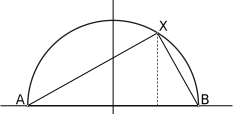
\includegraphics[width=144pt]{005Thales.pdf}
\end{center}
If $x$ is the $x$ coordinate of the point $X$, then what is its $y$ coordinate?  Find the components of the vectors $\tpv AX$ and $\tpv BX$.  Use the dot product to prove \textit{Thales' theorem}, i.e. show that $AXB$ is a right triangle. 
\answer
$X$ has coordinates $(x, \sqrt{1-x^2})$; 
${\tpv AX} = \vek 1+x \\ \sqrt{1-x^2} \tor $; 
${\tpv BX} = \vek x-1 \\ \sqrt{1-x^2}\tor$.

$\tpv AX \dpp \tpv BX = (1+x)  (x-1) + \bigl(\sqrt{1-x^2}\bigr)^2 =x^2-1 + 1-x^2 = 0$.  

So $\tpv AX$ and $\tpv BX$ are perpendicular.


\endanswer

\problem Compute %---Is the cross product associative?
\[
  \va = (\vi\cp\vj)\cp\vj 
  \text{ and }\vb = \vi\cp(\vj\cp\vj).
\]
What does your answer say about the associative property for the cross product?
(See \S~\ref{sec:cross-product-algebraic-properties}.)

What about
\[
  \vc = (\vi\cp\vj)\cp\vk  
  \text{ and }\vd = \vi\cp(\vj\cp\vk)?
\]


\problem Which of the following vector equations are true for any pair  
of vectors $\va$ and $\vb$?  Either give a proof (using the algebraic
properties or the algebraic or geometric descriptions).

\subprob $(\va+\vb)\dpp(\va-\vb) = \|\va\|^2 - \|\vb\|^2$~?  
\answer  
True:
\begin{align*}
  (\va+\vb)\dpp(\va-\vb) &=(\va+\vb) \dpp \va  - (\va+\vb) \dpp\vb\\
  &= \va \dpp \va +\vb \dpp \va  - \va \dpp\vb - \vb \dpp\vb\\
  &= \|\va\|^2 + \| \vb \|^2.
\end{align*}
\endanswer

\subprob  If  $\va\perp\vb$ then $\|\va+\vb\|^2 = \|\va\|^2 + \|\vb\|^2$~?% 
\answer  
True:  This is Pythagoras' theorem.  Here is an algebraic derivation:
\begin{align*}
  \|\va+\vb\|^2 &= (\va+\vb) \dpp (\va+\vb)\\
  &= (\va+\vb) \dpp \va  + (\va+\vb) \dpp\vb\\
  &= \va \dpp \va +\vb \dpp \va  + \va \dpp\vb + \vb \dpp\vb\\
  &= \|\va\|^2 + 2 \va \dpp\vb + \| \vb \|^2\\
  &= \|\va\|^2 + \| \vb \|^2.
\end{align*}
\endanswer

\subprob If  $\va\perp\vb$ then $\|\va-\vb\|^2 = \|\va\|^2 - \|\vb\|^2$  ~?%
\answer  
Not so.
The same computation as for the previous problem shows
\begin{align*}
  \|\va - \vb\|^2 &= (\va-\vb) \dpp (\va-\vb)\\
  &= (\va-\vb) \dpp \va  - (\va-\vb) \dpp\vb\\
  &= \va \dpp \va -\vb \dpp \va  - \va \dpp\vb + \vb \dpp\vb\\
  &= \|\va\|^2 - 2 \va \dpp\vb + \| \vb \|^2\\
  &= \|\va\|^2 + \| \vb \|^2.
\end{align*}
Therefore
\[
\|\va-\vb\|^2 = \|\va\|^2 - \|\vb\|^2
\]
only is true if $\vb=\vvv0$.
\endanswer

%%\problem ``Cramer's rule.''  Suppose we have to find solutions $x$,
%%$y$, $z$, of the following linear equations:
%%\begin{align*}
%%  a_1x+b_1y+c_1z & = d_1 \\
%%  a_2x+b_2y+c_2z & = d_2 \\
%%  a_3x+b_3y+c_3z & = d_3
%%\end{align*}
%%
%%\subprob Show that you can write these equations as
%%\[
%%x\va + y\vb + z\vc = \vd
%%\]
%%for certain vectors $\va$, $\vb$, $\vc$, and $\vd$.
%%
%%\subprob Show how you can get a formula for $x$ by taking the dot
%%product of both sides in the equation $x\va + y\vb + z\vc = \vd$ with
%%the vector $\vb\cp\vc$.
%%
%%\subprob How would you get a similar formula for $y$?  Or $z$?



\problem True or False:  

\subprob If $\va\perp\vb$ and also $\vb\perp\vc$ then $\va\perp\vc$ ?  

\subprob If $\va\perp\vb$ and also $\va\perp\vc$ then $\va\perp(\vb+\vc)$ ?  

\subprob If $\va\perp\vb$ and also $\vb\perp\vc$ then $\vb\perp(\va-\vc)$ ?  

\subprob If $\va\perp\vb+\vc$ and also $\va\perp\vb-\vc$ then $\va\perp\vb$ ?  

\problem Simplify the following expressions  

\subprob \(  (\va+\vb)\cp(\va+\vb) \)  
\answer  
\(  (\va+\vb)\cp(\va+\vb) =\vvv0 \)
\endanswer
%
\subprob \(  (\va+\vb+\vc)\cp(\va+\vb+\vc) \)  
\answer  
\(  (\va+\vb+\vc)\cp(\va+\vb+\vc) =\vvv0 \)
\endanswer
%
\subprob \(  (\va-\vb)\cp(\va+\vb) \)  
\answer  
\(
    (\va+\vb)\cp(\va-\vb) = 2\va\cp\vb.
\)
\endanswer
%
\subprob $(\va+\vb-\vc) \cp (\va-\vb+\vc)$  

\subprob $(\va+\vb-\vc) \dpp (\va-\vb+\vc)$  

\problem  
This problem is about ``cross division,'' i.e.~can you solve
$\va\cp\vb=\vc$ for $\vb$ if you know $\va$ and $\vc$?

\subprob Let  
\begin{equation*}
  \va =\ves1-\ves3,\qquad
  \vc = \ves1+3\ves2+2\ves3.
\end{equation*}
Find a vector $\vb$ for which $\va\cp\vb=\vc$, if there is such a thing.  (Hint:
if $\vc=\va\cp\vb$, then what do you know about $\va\dpp\vc$?)
\answer  
$\va\dpp\vc=\va\dpp(\va\cp\vb) =0$, but for the two given vectors in the problem
$\va\dpp\vc = -1\neq0$, so there cannot be a vector $\vb$ with $\va\cp\vb=\vc$
as $\vc$ is not perpendicular to $\va$.
\endanswer

\subprob Let $\va = 2\ves1-\ves3$, and $\vc = \ves1+3\ves2+2\ves3$.  
Find a vector $\vb$ for which $\va\cp\vb=\vc$, if such a thing exists. %
\answer  
In this case $\va\perp\vc$, so the argument from the first part of this problem
doesn't rule out that there might be a solution.  So let's try $\vb =
\tvek b_1\\b_2\\b_3\ttor$.  Then
\[
  \va\cp\vb
  = \vek b_2 \\ -b_1-2b_3 \\ 2b_2\tor \stackrel?= \vc
  = \vek 1\\3\\2\tor.
\]
Solving this for $b_1$, $b_2$, and $b_3$ leads to $b_2=1$, and $-b_1-2b_3=3$ as
only remaining equation.  Since we have found $b_2$ there are still two unknowns
left.  We can choose an arbitrary $b_3$ and set $b_1 = -3-2b_3$, e.g.~$b_3=0$
works, provided we choose $b_1 = -3$.
\endanswer

\problem \label{prb:law-of-cosines-and-dotprod}  
The \textit{law of cosines} says that in a triangle $\triangle ABC$
for which you know the sides $AB$ and $AC$, as well as the angle
$\angle A$, the length of the opposing side $BC$ is given by
\[
  (BC)^2 = (AB)^2 + (AC)^2  - 2(AB)(AC)\cos\angle A.
\]
Show how you can use the dot product to (re)prove this law.

Hint: consider the vector equation $\tpv BC = \tpv AC - \tpv AB$.  You will need
both the geometric description \eqref{eq:dotproduct-geometric} of the dot
product, and the algebraic properties from
\S~\ref{sec:dotproduct-algebraic-properties}.

\bigskip

\centerline{\bfseries Review problems}

\problem  Consider the points $A (1,1,2)$, $B(-1,-1,2)$, $C (1, -1, -1)$, and $D (-1, 1, -1)$.

\subprob
Find the distance from the point $A $ to the plane through the points $B$, $C$, and $D$.
\answer
First find the equation for the plane through $B, C, D$:  a normal vector for the plane is 
\[
  \vn = \tpv BC \times \tpv BD = \vek 2\\0\\-3\tor \times \vek 0\\ 2 \\ -3\tor =
  \vek 6 \\  6 \\ 4 \tor.
\]
We also need a point on the plane, we choose $B$ (could also have chosen $C$ or $D$). The equation for the plane then is $\vn\cdot\vx = \vn\cdot\vb$, i.e.
\[
  6x_1+6x_2+4x_3 = -6-6+8 = -4.
\]
The distance from the point $A$ to the plane is given by
\[
  \pm d = \frac{\vn \cdot(\va-\vb)}{\|\vn\|}
  =\frac1{\sqrt{6^2+6^2+4^2}} \vek 6\\6\\ 4 \tor \cdot \vek 1-(-1) \\1-(-1)\\2-2 \tor
  = \frac{10}{\sqrt{6^2+6^2+4^2}}
  = \frac {10}{\sqrt{88}}.
\]
\endanswer


\subprob
Find the cosine of the angle between the plane through $BCD$ and the $xy$-plane. (Hint: what is a normal to the $xy$-plane?)
\answer
The angle between two planes is the angle between their normals.  A normal to $BCD$ is the vector $\vn$ from part (a) of this problem.  A normal to the $xy$-plane is $\vk = \tvek0\\0\\1\ttor$.

The cosine of the angle between the two planes is
\[
  \cos \angle(BCD, xy\text{-plane})
  = \cos \angle(\vn, \vk)
  = \frac {\vn \cdot \vk}{\|\vn\|\, \|\vk\|}
  = \frac {4}{\sqrt{88} \cdot 1}
  = \frac {4}{\sqrt{88}}.
\]
\endanswer

\subprob Do the points $ A$ and $E (-1,-1,-1)$ lie on the same side of the plane $BCD$?
\answer
  The sign of $\vn\cdot(\vx-\vb)$ tells us if the point with position vector $\vx$ lies on the side of the plane $BCD$ that $\vn$ points to.  So to see if $A$ and $E$ are on the same side, we compare the signs of $\vn\cdot(\va-\vb)$ and $\vn\cdot(\ve-\vb)$.

  We have already computed $\vn\cdot(\va-\vb) = +10$; for the new point $E$ we have
  \[
    \vn\cdot(\ve-\vb) = \vek 6\\6\\4\tor \cdot \vek (-1)-(-1) \\(-1)-(-1)\\(-1)-2 \tor
    =4\cdot(-3) = -12.
  \]
   So $\vn\cdot(\va-\vb) = +10$ and $\vn\cdot(\ve-\vb) = -12$ have opposite signs, which means that $A$ and $E$ lie on opposite sides of the plane $BCD$.
\endanswer


\subprob  Find a parametric representation for the line through $A$ and $C$, and determine where this line intersects the three coordinate planes (i.e.~the $xy$-plane, the $yz$-plane, and the $xz$-plane).
\answer
  The direction of the line is given by the vector $\tpv AC = \vc-\va = \tvek 0 \\ -2 \\ -3\ttor$.

  A parametrization of the line is then given by
  \[
    \vx = \va + t\tpv AC = 
    \vek 1 \\ 1 \\ 1 \tor + t \vek 0 \\ -2 \\ -2 \tor
    = \vek 1 \\ 1-2t \\ 1-2t \tor.
  \]
  
  We see that $\vx$ lies on the $xy$ plane when its third component vanishes, i.e.~when $1-2t=0$.  This happens for $t=\frac12$.  The point where the line intersects the $xy$-plane is therefore $(1, 0, 0)$.  

  To see where the line intersects the $xz$-plane, we check when the second component of $\vx$ vanishes.  The second component is the same as the third, namely $1-2t$, so we again get $t=\frac12$, and the intersection point is $(1, 0, 0)$.

  Finally, the first component of $\vx$ is $1$ for all values of $t$, so it never vanishes.  This line does not intersect the $yz$-plane.

\endanswer

\problem Let two points $A(2, 2, 1)$ and $B(2,0,3)$ be given.
Find an equation for the plane through $A$, $B$, and the origin.

\answer
We have three points on the plane $A$, $B$, and the origin $O (0,0,0)$
From these we compute a normal
\[
\vn = \tpv OA \times \tpv OB
= \vek 2\\2\\1\tor \times \vek 2\\0\\3\tor
= \vek -1 \\ -4 \\ -4 \tor.
\]
The equation for the plane is then $\vn\cdot\vx = \vn\cdot\vp$, where $\vp$ is the position vector of any point we know to be on the plane:  we can choose $\vp$ to be either $\tpv OA$, $\tpv OB$, or $\vvv0$ (the position vector of the origin).  We choose $\vp=\vvv0$ because that is the easiest, but the other choices should give the same answer.  Thus we find the equation for the plane to be
\[
-x_1 -4x_2-4x_3=0.
\]
If you don't like all the minus signs, then you can multiply both sides with $-1$, which gives you $x_1+4x_2+4x_2=0$.

\endanswer





% vim: fdc=3 columns=90 fdm=expr
